% ars_intro_methods.tex -- independent ARS draft_writer_agent draft of Sections I and II (2026-10-07).
% Drop-in fragment for main.tex: replaces the text from \section{Introduction} up to \section{Results}.
% Facts traced to protocol/SEVERITY-SWEEP-SPEC.md, protocol/STATISTICS-PLAN.md, protocol/CFD-ARM-SPEC.md,
% code/{zerod_ffr,error_types,ablation,severity_sweep,analyse_ablation}.py and the task brief (3D case study).
% ---------------------------------------------------------------------------------------------------------------
\section{Introduction}
\IEEEPARstart{F}{ractional} flow reserve (FFR), the ratio of mean pressure distal to a coronary stenosis to aortic
pressure during maximal hyperaemia, guides revascularisation: lesions with FFR $\leq 0.80$ are treated, and
FFR-guided intervention improves outcomes over angiographic guidance \cite{tonino2009}. FFR can also be computed
without a pressure wire. A lumen segmented from coronary computed tomography angiography (CCTA) is converted into a
blood-flow model, and the computed FFR has been validated against invasive measurement in multicentre trials
\cite{taylor2013,norgaard2014}. Three-dimensional (3D), reduced-order and learned formulations of this calculation
exist \cite{kim2010,itu2016}.

Every such model needs boundary conditions, the pressures, flows or resistances imposed at the model's inlet and
outlets to represent the circulation that the image does not resolve. The largest part of this circulation is the
microvascular bed, the arterioles and capillaries downstream of the segmented arteries that set how much flow each
myocardial territory draws. Its resistance is not measured. It is derived from the segmented lumen itself, usually
through scaling laws that link vessel size to supplied flow or myocardial mass \cite{murray1926,choy2008}, and it is
increasingly tuned so that the model reproduces perfusion measured by imaging \cite{menon2024}. The segmentation
therefore enters the computed FFR twice: through the resistance of the arteries and through the boundary conditions
derived from them.

The effect of segmentation error has been studied mainly as calibre error, a lumen that is too wide or too narrow
with the branching structure unchanged. Published sensitivity analyses perturb the lumen radius at fixed
bifurcations and report a continuous change in FFR \cite{sankaran2015tmi,sankaran2015cmame,fernandez2024,dalmaso2025}.
Studies that set geometry against boundary conditions rank the two by their influence on a continuous output
\cite{sankaran2016,tanade2022,colebank2019,korte2023}. Topological error, a change in the branching structure such
as a missed side branch or a vessel that ends too early, has received less attention, although vessel breaks occur
in the output of current coronary segmentation methods that score highly on overlap metrics \cite{bransby2026}.
The evidence on side branches is also divided. With outlet resistance held fixed, the loss of a side branch shifted
computed FFR by 13--15\% in models built from optical coherence tomography \cite{gamage2022}. When the microvascular
resistance was re-tuned, a change in side-branch flow altered diagnostic accuracy little \cite{gosling2020}. A change
of outlet model in a clinical cohort left the area under the curve unchanged while sensitivity moved
\cite{fossan2026}.

These results leave one question open. If the boundary conditions are tuned until the model matches measured
perfusion, a topological error may disappear from the validation check while it remains in the pressure field. The
studies above report continuous sensitivity or aggregate accuracy, and none compares fixed, re-derived and tuned
boundary conditions on the same corrupted anatomy at the 0.80 decision threshold. Whether a model can pass a
perfusion check and still assign the wrong treatment class has therefore not been tested.

We address this question with a controlled ablation. We inserted stenoses into real coronary trees so that baseline
FFR spans the decision threshold, applied two topological and two calibre error types, and recomputed FFR with a
reduced-order model under three boundary-condition protocols and two microvascular bed structures. The contributions
are (1) an error model that separates topological from calibre segmentation error, with calibre magnitudes taken
from measured inter-observer disagreement; (2) a paired comparison of fixed, re-derived and perfusion-tuned boundary
conditions at the 0.80 threshold, set against the variability of repeat invasive measurement; and (3) a 3D case
study that tests the mechanism at higher fidelity on one lesion.

% ---------------------------------------------------------------------------------------------------------------
\section{Methods}
Fig.~\ref{fig:design} summarises the design. The cohort, the error types, the protocols and the analysis plan were
fixed, and the cohort list was hashed (SHA-256), before the ablation was run.

\begin{figure*}[!t]\centering
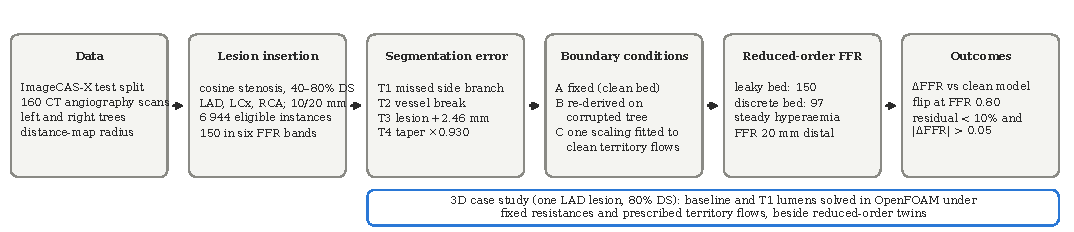
\includegraphics[width=\textwidth]{figures/fig1_design.pdf}
\caption{Study design. Stenoses of 40--80\% diameter stenosis (DS) were inserted into coronary trees from the
ImageCAS-X test split, four segmentation error types were applied to each instance, and FFR was recomputed with a
reduced-order model under three boundary-condition protocols and two microvascular bed structures. One instance was
also solved in three dimensions.}
\label{fig:design}
\end{figure*}

\subsection{Data and Cohort}
We used ImageCAS-X \cite{bransby2026,imagecasx_data}, which adds voxel lumen labels, labelled coronary centrelines and
scan descriptors to CCTA scans from ImageCAS \cite{zeng2023}. All instances came from the dataset's 160-scan test
split. The vessel radius at each centreline point was the Euclidean distance from the point to the lumen boundary in
the mask, less half a voxel, smoothed along each segment. The dataset contains few lesions near the decision
threshold, so we inserted one stenosis per instance into an otherwise unchanged tree.

A host vessel (left anterior descending, LAD; left circumflex, LCx; or right coronary artery, RCA) was eligible if
image quality was at least 2 on the dataset's four-point scale, the healthy reference radius at the lesion centre
was at least 1.0~mm, native disease between the lesion and the measurement point was below 40\% DS, and the
pre-insertion FFR was at least 0.90. The measurement point lay 20~mm distal to the lesion's distal edge, as for a
pressure wire, on a vessel of radius at least 0.75~mm. The lesion was an axisymmetric cosine narrowing,
\begin{equation}
\begin{aligned}
r_\mathrm{new}(s)&=\min\!\big(r,\;(1-w)\,r+w\,r_\mathrm{fit}(1-\mathrm{DS})\big),\\
w(s)&=\tfrac12\big[1+\cos\big(\pi\,(s-c)/(L/2)\big)\big],
\end{aligned}
\end{equation}
for $|s-c|<L/2$, where $s$ is arc length, $c$ the lesion centre, $L$ its length and $r_\mathrm{fit}$ the healthy
reference radius from a robust linear taper fit. The vessel was never widened. Lesions were centred 20 or 45~mm from
the vessel origin, were 10 or 20~mm long and had 40, 50, 55, 60, 65, 70, 75 or 80\% DS. The microvascular bed and the
flow demand were computed from the original tree and held fixed, so the lesion changed the epicardial radius only.

The full factorial gave 6\,944 instances on 280 host vessels from 140 scans. From these we drew 25 instances in each
of six 0.05-wide bands of baseline FFR from 0.65 to 0.95, with at most two instances per tree, giving 150 instances
(50 per vessel) in 108 trees from 93 patients.

\subsection{Reduced-Order FFR Model}
The model places a node at every centreline point. Each element between consecutive nodes has the Poiseuille
resistance $8\mu\,\Delta s/(\pi r^4)$ of the actual radius, with viscosity $\mu = 0.004$~Pa\,s. Where the narrowing
exceeds 30\% DS, an expansion loss $\Delta p = K\,Q|Q|$ is added at the throat, with
$K = \rho K_t/(2A_0^2)\,(A_0/A_s-1)^2$, $K_t = 1.52$, density $\rho = 1060$~kg\,m$^{-3}$, and $A_0$ and $A_s$ the
reference and throat areas. The aortic pressure is 90~mmHg and the venous pressure 5~mmHg. The nonlinear system is
solved by under-relaxed fixed-point iteration to a relative flow change below $10^{-8}$, and the mass-conservation
error is recorded for every solve. FFR is the computed pressure at the measurement point divided by aortic pressure.
The model is steady and represents hyperaemia without autoregulation.

The microvascular bed was modelled as a conductance from network nodes to venous pressure, in two structures that
differ in how a deleted vessel is treated. In the leaky bed, every node of the tree truncated at a reference radius
of 0.50~mm carries a conductance proportional to its reference radius cubed less that of its children. This
distributed outflow represents unresolved side branches \cite{gosling2020} and returns the conductance of a deleted
branch as outflow at its parent node. In the discrete bed, conductance sits only at the outlets of the tree truncated
at 0.60~mm, weighted by the outlet radius to the power 2.66, the scaling of myocardial mass with vessel size
\cite{choy2008}. This is the outlet structure that a 3D model can represent. In both structures one bed constant was
calibrated on the healthy-equivalent network, the tree with its reference radius and no lesion, so that inflow equals
the hyperaemic demand $Q = k\,r_\mathrm{in}^3$ with $k = 562$~s$^{-1}$ \cite{murray1926}. The leaky bed was analysed
on all 150 instances. The discrete bed was analysed on the 97 instances whose healthy-equivalent network had a
main-vessel FFR of at least 0.90 and at least two outlets. Baseline FFR bands were derived separately for each bed.
Halving the centreline spacing changed FFR by at most 0.005 in either bed.

\subsection{Segmentation Error Types}
Each error type was applied to the clean tree with the lesion in place (Table~\ref{tab:design}). Two are topological,
changing which vessels exist, and two are calibre errors, changing lumen size or lesion extent with the branching
unchanged. The missed side branch (T1) deletes the largest branch leaving the host vessel distal to the lesion,
together with its subtree. The vessel break (T2) ends the host vessel 25~mm beyond the lesion's distal edge, so the
measurement point survives and the run-off beyond it is lost. The lesion-length error (T3) re-inserts the same
stenosis 2.46~mm longer. The taper error (T4) multiplies the radius by 0.930 from the lesion's proximal shoulder
distally and in every descendant vessel, with the truncation radius scaled by the same factor so that no outlet is
removed by the error.

The calibre magnitudes come from the ImageCAS-X re-annotation of the test split. The 95th-percentile surface distance
between annotators (2.46~mm) sets T3. The lumen Dice coefficient of 92.8\% sets T4, as the radius ratio $k$ of two
coaxial cylinders with $2k^2/(k^2+1) = 0.928$. Because both annotators edited the same automatically generated
centrelines, these statistics are an upper bound on agreement. The magnitudes of T1 and T2 are design choices. Nodes
of the corrupted tree were matched to the clean tree by coordinate, and FFR was read at the same anatomical point.

\begin{table}[!t]
\caption{Segmentation Error Types and Boundary-Condition Protocols}
\label{tab:design}
\centering\footnotesize
\begin{tabular}{@{}p{0.9cm}p{4.0cm}p{2.3cm}@{}}
\toprule
 & Definition & Magnitude (source)\\
\midrule
T1 & Missed side branch: largest branch distal to the lesion deleted with its subtree (topological) & Largest eligible branch (design choice)\\
T2 & Vessel break: host vessel ended beyond the measurement point (topological) & 25~mm past lesion edge (design choice)\\
T3 & Lesion length over-estimated (calibre) & $+2.46$~mm (inter-observer HD95)\\
T4 & Lumen under-sized from the lesion distally (calibre) & Radius $\times 0.930$ (inter-observer DSC)\\
\midrule
A & Fixed: surviving nodes keep the clean bed conductances & --\\
B & Re-derived: bed rule and demand recomputed on the corrupted tree & --\\
C & Tuned: one bed scaling fitted to the clean territory flows & One parameter, $\geq 2$ targets\\
\bottomrule
\end{tabular}
\\[2pt]
\parbox{\columnwidth}{\footnotesize HD95: 95th-percentile Hausdorff distance. DSC: Dice similarity coefficient.}
\end{table}

\subsection{Boundary-Condition Protocols}
Each corrupted tree was solved under three protocols. Under Protocol A (fixed), surviving nodes keep the
conductances of the clean model and the bed of deleted nodes is lost. It describes the case in which the boundary
conditions were obtained correctly despite the segmentation error. Under Protocol B (re-derived), the bed rule is
applied to the corrupted tree and the bed constant is recalibrated to that tree's own demand, as an automated
pipeline does with whatever anatomy it receives.

Under Protocol C (tuned), one global scaling of the bed is fitted so that the corrupted model reproduces the clean
model's territory flows. A territory is the subtree below each child of the first bifurcation of the clean tree, and
its target is the total bed outflow of that subtree in the clean model, including the share of any vessel the error
deleted, because the myocardium is perfused whether or not its artery was segmented. Each corrupted node belongs to
the territory of its clean counterpart. The fit minimised the mean squared relative error of the territory flows,
using a 61-point grid over $\pm 1.5$ decades of the bed constant followed by bounded refinement. A fit at the edge of
the search range was recorded as a failure. One parameter against two or more targets makes the fit over-determined
and the tuning the least flexible a pipeline could use. Protocol C was therefore defined only when at least two
territories retained a vessel.

For every protocol we computed the territory-perfusion residual, the root mean square of the relative differences
between the model's territory flows and the clean targets. It is the quantity a perfusion check compares.

\subsection{Three-Dimensional Case Study}
One instance, scan 14 with a 20~mm, 80\% DS lesion in the proximal LAD, was solved in three dimensions in three
lumens: without the lesion, with the lesion (baseline), and with the lesion and T1. The lumen surface was generated
from the segmentation mask. The lesion was applied by moving surface vertices radially with the cosine law of
(1), and the branch was removed by deleting its voxels before surface extraction. Meshes of 3.5--3.9 million cells
were generated with cfMesh, with 25~\textmu m cells in a throat zone extending $\pm 4$~mm and four boundary layers. Steady
laminar flow of a Newtonian fluid with the same viscosity and density was solved in OpenFOAM (ESI v2406) with rigid
walls and the aortic pressure at the inlet. The outlets received either the clean model's resistances (Protocol A) or
prescribed clean territory flows, distributed over the surviving outlets of each territory in proportion to their
bed weights (the per-outlet form of Protocol C). FFR was the area-averaged pressure on a cross-section at the measurement point divided by aortic
pressure. A grid study on an idealised 70\% DS stenosis gave a discretisation uncertainty of $5.5\times10^{-4}$ in
FFR. For comparison, a reduced-order twin was rebuilt on the area-equivalent radius of the meshed lumen and solved
with the same outlet conditions.

\subsection{Outcomes and Statistical Analysis}
For each instance, error type, protocol and bed, $\Delta$FFR was the corrupted model's FFR minus that of the
instance's own clean model in the same bed. A flip was a change of classification at FFR 0.80 between the two. A
model passed the perfusion check when its residual was below 10\%. This threshold is stricter than the 13--16\%
expected when a deterministic model output is compared with one regional perfusion measurement at published
repeatability \cite{schindler2023,brown2018}, and a looser threshold can only increase the number of models that
pass. An FFR error was material when $|\Delta\mathrm{FFR}| > 0.05$. The thresholds of 13\% and 16\% were analysed as
sensitivities.

Proportions are reported with Wilson 95\% confidence intervals (CIs). Protocol contrasts (B against A, C against A,
C against B) were paired within instance and tested with the exact McNemar test, with Holm correction across the
three contrasts of each error type and bed. Topological and calibre errors were compared with a paired sign test on
the per-instance mean flip rate of each class. Paired differences in $|\Delta\mathrm{FFR}|$ were tested with the
Wilcoxon signed-rank test. As a reference for flips that measurement alone would produce, we computed for each
instance the probability that a repeat invasive FFR, drawn from a normal distribution centred on the clean value with
the published repeat-measurement standard deviation of 0.018 \cite{johnson2015}, falls on the other side of 0.80
\cite{petraco2013}. A mixed logistic model of flip on error type, protocol, severity, length and band, with random
intercepts for patient and lesion slot, was fitted as a variational-Bayes binomial model, with a generalised
estimating equation model clustered on patient beside it. Because the two beds differ in structure, each analysis
was run in both, effect sizes are reported per bed, and a finding is claimed only where its direction agreed in
both.

Three changes from the analysis plan were made. The plan specified a frequentist mixed logistic model, which was not
available in the fixed software environment. A sensitivity analysis with one bed scaling per territory was not run.
The measurement-noise reference was computed per instance from the repeat-measurement standard deviation. The plan also specified a 3D replication on
30 instances and a detector of concealed error. Their results are not part of this report. Analyses used Python
(NumPy, SciPy, pandas and statsmodels).
